\chapter{Arhitektura i dizajn sustava}
		 Izbor odgovarajuće arhitekture programske poruke jedan je od najbitnijih koraka u oblikovanju sustava jer ona predstavlja poveznicu između zahtjeva na sustav i same implementacije sustava. Dobra arhitektura povlači dobru fleksibilnost sustava, jednostavnu mogućnost nadogradnje i jeftino održavanje.
		

\noindent S obzirom na to da je zadatak ovog projekta napraviti aplikaciju za šahovski klub, logičan izbor je web aplikacija. Primarni razlog je to što web aplikacija ne ovisi o platformi, već radi na svakom sustavu koji ima web preglednik što znatno smanjuje vrijeme i troškove potrebne za razvoj za više platformi
		

\noindent Radni okvir koji smo odabrali za arhitekturu je Django (pisan u i za jezik Python). S njime smo arhitekturu sustava odlučili temeljiti na MVT (Model-View-Template) konceptu kojeg on nativno podržava. Jedina bitna razlika između njega i poznatog MVC (Model-View-Controller) koncepta je to što u Django sam po sebi sređuje "controller" dio (programski kod koji kontrolira interakciju između modela i viewa) i daje nam na raspolaganje Template.
		
		Dakle aplikacija se sastoji od 3 dijela:
		\begin{itemize}
			\item 	Model - Sređuje apstrakciju podataka, služi kao sučelje za podatke spremljene u bazu i dopušta upravljanje njima bez prevelikog razumijevanja kompleksnosti same baze 
			\item 	View - funkcionalnosti slične controlleru u MVC konceptu. Sređuje svu logiku koja se treba prikazati na templateu i služi kao "most" između modela i templatea
			\item 	Template - funkcionalnosti slične Viewu u MVC konceptu. Služi kao sloj prikaza sadržaja i zadužen je za to kako i što će biti prikazano korisniku. Specifično za Django, Template je vrsta HTML datoteke koja može koristiti Django Template Language (DTL) što nam znatno olakšava komunikaciju između frontenda i backenda aplikacije.	
		\end{itemize}
		

				
		\section{Baza podataka}
		
		Za sustav baza podataka za ovaj projekt smo odabrali PostgreSQL. 
		
		PostgreSQL je objektno-relacijski sustav upravljanja bazama podataka (ORDBMS) zasnovan na POSTGRES-u, inačica 4.2, razvijen na Kalifornijskom sveučilištu na Odjelu za računalne znanosti Berkeley. POSTGRES je pionir mnogih koncepata koji su tek kasnije postali dostupni u nekim komercijalnim sustavima baza podataka.
		
		PostgreSQL je "open-source" potomak ovog izvornog Berkeley koda. Podržava velik dio SQL standarda i nudi brojne moderne značajke poput:
		\begin{packed_item}
			\item složenih upita,
			\item stranih ključeva,
			\item okidača,
			\item obnovljivih pogleda,
			\item transakcijski integritet te
			\item multiverzijski protokol kontrole istodobnog
			pristupa
		\end{packed_item}
		
		Također, korisnik može proširiti PostgreSQL na mnogo načina, na primjer dodavanjem novih:
		\begin{packed_item}
			\item vrsta podataka,
			\item funkcija,
			\item operatora,
			\item agregatnih funkcija,
			\item indeksnih metoda te
			\item proceduralnih jezika.
		\end{packed_item}
		
		
		A zbog liberalne licence, PostgreSQL može koristiti, mijenjati i distribuirati bilo tko u bilo koju svrhu, bilo privatnu, komercijalnu ili akademsku.\footnote{\url{https://www.postgresql.org/docs/current/intro-whatis.html}}
		
		U relacijskim bazama podataka, osnovne gradivne jedinice su tablice. Tablice koje grade bazu podataka ovog projekta su:
		\begin{packed_item}
			\item taktika
			\item rjesenjeTaktika
			\item dojavaPogreske
			\item view - rangLista
			\item Korisnik
			\item Grupa
			\item Novost
			\item Trening
			\item turnir
			\item PrijavaTrening
			\item PrijavaTurnir
			\item Transakcija
			
		\end{packed_item}
		
		\eject
		
			\subsection{Opis tablica}
			Primarni ključevi tablice označeni su sa slovom 'P', a strani ključevi sa slovom 'F'.\\
			
			\noindent Entitet \textbf{Taktika} u odnosu je \textit{One to Many} s entitetima \textbf{Rješenje taktika} i \textbf{Dojava pogreške}.
				\begin{longtabu} to \textwidth {|X[6, l]|X[6, l]|X[20, l]|}
					
					\hline \multicolumn{3}{|c|}{\textbf{taktika}}	 \\[3pt] \hline
					\endfirsthead
					
					\hline \multicolumn{3}{|c|}{\textbf{taktika}}	 \\[3pt] \hline
					\endhead
					
					\hline 
					\endlastfoot
					
					\cellcolor{LightGreen}idTaktika P& INT	   &  identifikacijski broj taktike	\\ \hline
					createdAt	& TIMESTAMP &   vrijeme stvaranja taktike, služi za kronološko sortiranje taktika	\\ \hline 
					\cellcolor{LightBlue}idUser F& INT & identifikator trenera ili admina koji je stvorio taktiku  \\ \hline 
					initConfig & VARCHAR (100)	&  string koji opisuje inicijalno stanje šahovske ploče	\\ \hline 
					movesWhite & VARCHAR (3000) & string koji opisuje poteze bijelih figurica \\ \hline
					movesBlack & VARCHAR (3000) & string koji opisuje poteze crnih figurica \\ \hline
					tezina & DECIMAL & težina taktike, koristi se u računanju bodova, u rasponu od 1 do 3 \\ \hline
					brojGlasova & INT & broj korisnika koji su glasali za neku težinu taktike \\ \hline

				\end{longtabu}
				
				\noindent Entitet \textbf{Rješenje taktika} u odnosu je \textit{One to One} s entitetnom \textbf{Taktika}, te u odnosu  \textit{One to One} s entitetnom \textbf{Korisnik}.
				\begin{longtabu} to \textwidth {|X[6, l]|X[6, l]|X[20, l]|}
					
					\hline \multicolumn{3}{|c|}{\textbf{rjesenjeTaktika}}	 \\[3pt] \hline
					\endfirsthead
					
					\hline \multicolumn{3}{|c|}{\textbf{rjesenjeTaktika}}	 \\[3pt] \hline
					\endhead
					
					\hline 
					\endlastfoot
					
					\cellcolor{LightGreen}idTaktika PF& INT	   &  identifikacijski broj taktike koja je rješena, foreign key	\\ \hline
					\cellcolor{LightGreen}idUser PF& INT & identifikator člana koji je riješio taktiku, foreign key  \\ \hline 
					vrijeme & DECIMAL & vrijeme rješavanja taktike u minutama \\ \hline
					
				\end{longtabu}
				\eject
				
				\noindent Entitet \textbf{Dojava pogreške} u odnosu je \textit{One to One} s entitetnom \textbf{Taktika}, te u odnosu  \textit{One to One} s entitetnom \textbf{Korisnik} koji je prijavio taktiku. Također je u odnosu \textit{One to One} s entitetnom \textbf{Korisnik} koji predstavlja trenera koji je zadužen za revidiranje dojave.
				\begin{longtabu} to \textwidth {|X[6, l]|X[6, l]|X[20, l]|}
					
					\hline \multicolumn{3}{|c|}{\textbf{dojavaPogreske}}	 \\[3pt] \hline
					\endfirsthead
					
					\hline \multicolumn{3}{|c|}{\textbf{dojavaPogreske}}	 \\[3pt] \hline
					\endhead
					
					\hline 
					\endlastfoot
					
					\cellcolor{LightGreen}idDojava P& INT	   &  identifikacijski broj dojave o pogrešci	\\ \hline
					\cellcolor{LightBlue}idTaktika F& INT	   &  identifikacijski broj prijavljene taktike	\\ \hline
					\cellcolor{LightBlue}idUserDojavio F& INT & identifikator člana koji je dojavio pogrešku na taktiku  \\ \hline 
					\cellcolor{LightBlue}idUserRevidira F& INT & identifikator trenera koji revidira dojavu  \\ \hline 
					prihvacena & BOOLEAN	&  je li dojava prihvaćena ili odbačena, NULL znači da čeka na revidiranje	\\ \hline 
					predlozeniTijek & VARCHAR (6000) & string koji opisuje poteze koje je predložio član koji je dojavio pogrešku \\ \hline
					opisPoteza & TEXT & opis poteza koje je član unio \\ \hline
					
				\end{longtabu}
				
				\noindent Entiteti u tablici \textbf{rangLista} u odnosu su \textit{One to One} s entitetnom \textbf{Korisnik}.
				\begin{longtabu} to \textwidth {|X[6, l]|X[6, l]|X[20, l]|}
					
					\hline \multicolumn{3}{|c|}{\textbf{view - rangLista}}	 \\[3pt] \hline
					\endfirsthead
					
					\hline \multicolumn{3}{|c|}{\textbf{view - rangLista}}	 \\[3pt] \hline
					\endhead
					
					\hline 
					\endlastfoot
					
					\cellcolor{LightGreen}idUser PF& INT	   &  identifikacijski broj člana	\\ \hline
					username & VARCHAR	   &  korisničko ime člana	\\ \hline
					bodovi & INT & broj bodova koje je član sveukupno osvojio \\ \hline 
					
				\end{longtabu}
			
				\noindent Entitet \textbf{Korisnik} u odnosu je \textit{One to Many} s entitetima \textbf{Rješenje taktika, Grupa} i \textbf{Dojava pogreške}, te u odnosu \textit{One to One} s entitetima iz tablice \textbf{rangLista}.
				\begin{longtabu} to \textwidth {|X[6, l]|X[8, l]|X[20, l]|}
					
					\hline \multicolumn{3}{|c|}{\textbf{Korisnik}}	 \\[3pt] \hline
					\endfirsthead
					
					\hline \multicolumn{3}{|c|}{\textbf{Korisnik}}	 \\[3pt] \hline
					\endhead
					
					\hline 
					\endlastfoot
					
					\cellcolor{LightGreen} idUser P& INT &  identifikacijski broj člana \\ \hline
					\cellcolor{LightBlue} idGrupa F& INT & identifikacijski broj grupe \\ \hline
					username & VARCHAR (20) &  korisničko ime člana \\ \hline 
					password & VARCHAR (20) & lozinka člana \\ \hline 
					email & VARCHAR (20) & mail adresa člana \\ \hline
					ime & VARCHAR (20) & ime člana \\ \hline
					prezime & VARCHAR (20) & prezime člana \\ \hline
					
				\end{longtabu}
			
				\begin{longtabu} to \textwidth {|X[6, l]|X[8, l]|X[20, l]|}
				
					\hline \multicolumn{3}{|c|}{\textbf{Grupa}}	 \\[3pt] \hline
					\endfirsthead
					
					\hline \multicolumn{3}{|c|}{\textbf{Grupa}}	 \\[3pt] \hline
					\endhead
					
					\hline 
					\endlastfoot
					
					\cellcolor{LightGreen} idGrupa P& INT & identifikacijski broj grupe \\ \hline
					imeGrupe & VARCHAR (20) &  ime grupe \\ \hline
				
				\end{longtabu}
				
				\noindent Entitet \textbf{Novost} u odnosu je \textit{Many to One} s entitetom \textbf{Korisnik} 
				\begin{longtabu} to \textwidth {|X[10, l]|X[8, l]|X[20, l]|}
				
					\hline \multicolumn{3}{|c|}{\textbf{Novost}}	 \\[3pt] \hline
					\endfirsthead
					
					\hline \multicolumn{3}{|c|}{\textbf{Novost}}	 \\[3pt] \hline
					\endhead
					
					\hline 
					\endlastfoot
					
					\cellcolor{LightGreen} idUser PF& INT & identifikacijski broj autora \\ \hline
					\cellcolor{LightGreen} vrijemeObjavljivanja P& DATETIME & vrijeme i datum objavljivanja \\ \hline
					naslov & VARCHAR (50) & naslov novosti\\ \hline
					tekst & TEXT & tekst novosti\\ \hline
				
				\end{longtabu}

				\noindent Entitet \textbf{Trening} u odnosu je \textit{One to Many} s entitetom \textbf{PrijavaTrening}, te u odnosu \textit{Many to One}  s entitetom \textbf{Korisnik}.

				\begin{longtabu} to \textwidth {|X[10, l]|X[8, l]|X[20, l]|}
				
					\hline \multicolumn{3}{|c|}{\textbf{Trening}}	 \\[3pt] \hline
					\endfirsthead
					
					\hline \multicolumn{3}{|c|}{\textbf{Trening}}	 \\[3pt] \hline
					\endhead
					
					\hline 
					\endlastfoot
					
					\cellcolor{LightGreen} idTreninga P& INT & identifikacijski broj treninga\\ \hline
					\cellcolor{LightBlue} idOrganizatora F& INT & identifikacijski broj organizatora treninga \\ \hline
					vrijemePocetka & DATETIME & vrijeme i datum početka treninga\\ \hline
					vrijemeZavrsetka & DATETIME & vrijeme i datum završetka treninga\\ \hline
					opisTreninga & TEXT & opisan sadržaj treninga\\ \hline
				
				\end{longtabu}
				
				\noindent Entitet \textbf{Turnir} u odnosu je \textit{One to Many} s entitetom \textbf{PrijavaTurnir}.

				\begin{longtabu} to \textwidth {|X[10, l]|X[8, l]|X[20, l]|}
				
					\hline \multicolumn{3}{|c|}{\textbf{Turnir}}	 \\[3pt] \hline
					\endfirsthead
					
					\hline \multicolumn{3}{|c|}{\textbf{Turnir}}	 \\[3pt] \hline
					\endhead
					
					\hline 
					\endlastfoot
					
					\cellcolor{LightGreen} idTurnira P& INT & identifikacijski broj turnira\\ \hline
					formatTurnira & TEXT & opisan format turnira \\ \hline
					vrijemePocetka & DATETIME & vrijeme i datum početka turnira\\ \hline
					vrijemeZavrsetka & DATETIME & vrijeme i datum završetka turnira\\ \hline
					brojSudionika & INT & maksimalan broj sudionika na turniru\\ \hline
				
				\end{longtabu}

				\noindent Entitet \textbf{PrijavaTrening} u odnosu je \textit{Many to One} s entitetom \textbf{Trening}, te u odnosu \textit{One to One}  s entitetom \textbf{Korisnik}.

				\begin{longtabu} to \textwidth {|X[10, l]|X[8, l]|X[20, l]|}
				
					\hline \multicolumn{3}{|c|}{\textbf{PrijavaTrening}}	 \\[3pt] \hline
					\endfirsthead
					
					\hline \multicolumn{3}{|c|}{\textbf{PrijavaTrening}}	 \\[3pt] \hline
					\endhead
					
					\hline 
					\endlastfoot
					
					\cellcolor{LightBlue} idClana PF& INT & identifikacijski broj člana\\ \hline
					\cellcolor{LightBlue} idTreninga PF & INT & identifikacijski broj treninga \\ \hline
				
				\end{longtabu}

				\noindent Entitet \textbf{PrijavaTurnir} u odnosu je \textit{Many to One} s entitetom \textbf{Turnir}, te u odnosu \textit{One to One}  s entitetom \textbf{Korisnik}.

				\begin{longtabu} to \textwidth {|X[10, l]|X[8, l]|X[20, l]|}
				
					\hline \multicolumn{3}{|c|}{\textbf{PrijavaTurnir}}	 \\[3pt] \hline
					\endfirsthead
					
					\hline \multicolumn{3}{|c|}{\textbf{PrijavaTurnir}}	 \\[3pt] \hline
					\endhead
					
					\hline 
					\endlastfoot
					
					\cellcolor{LightBlue} idClana PF& INT & identifikacijski broj člana\\ \hline
					\cellcolor{LightBlue} idTurnira PF& INT & identifikacijski broj turnira \\ \hline
				
				\end{longtabu}
	
				\noindent Entitet \textbf{Transakcija} u odnosu je \textit{Many to One} s entitetom \textbf{Korisnik}.

				\begin{longtabu} to \textwidth {|X[10, l]|X[8, l]|X[20, l]|}
				
					\hline \multicolumn{3}{|c|}{\textbf{Transakcija}}	 \\[3pt] \hline
					\endfirsthead
					
					\hline \multicolumn{3}{|c|}{\textbf{Transakcija}}	 \\[3pt] \hline
					\endhead
					
					\hline 
					\endlastfoot
					
					\cellcolor{LightGreen} idTransakcije P& INT & identifikacijski broj transakcije\\ \hline
					\cellcolor{LightBlue} idClana F& INT & identifikacijski broj člana\\ \hline
					datumTransakcije & DATETIME & vrijeme i datum izvršavanja transakcije\\ \hline
					iznosUplate & DECIMAL & uplaćen iznos\\ \hline

				\end{longtabu}

				
			
			\subsection{Dijagram baze podataka}
			
			\begin{figure}[H]
					\centerfloat
        					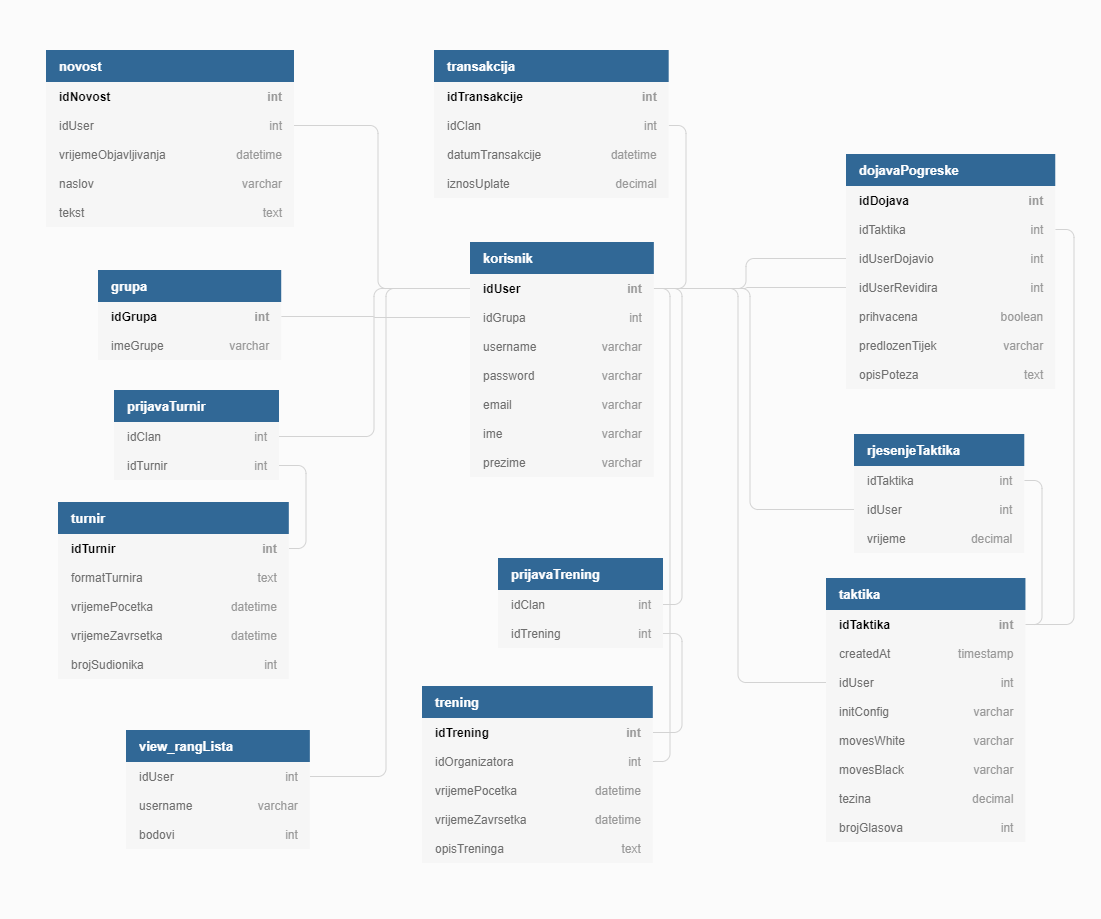
\includegraphics[scale=0.60]{dijagrami/dijagramBaze.png} %veličina slike u odnosu na originalnu datoteku i pozicija slike
        					\caption{E-R dijagram baze podataka}
        					\label{fig:DBdiagram}
				\end{figure}
			
			\eject
			
			
		\section{Dijagram razreda}

			\text{Dijagram modela potrebnih za funkcionalnosti autentikacije.}
			\begin{figure}[H]
					\centerfloat
					\advance\leftskip0.7cm
        					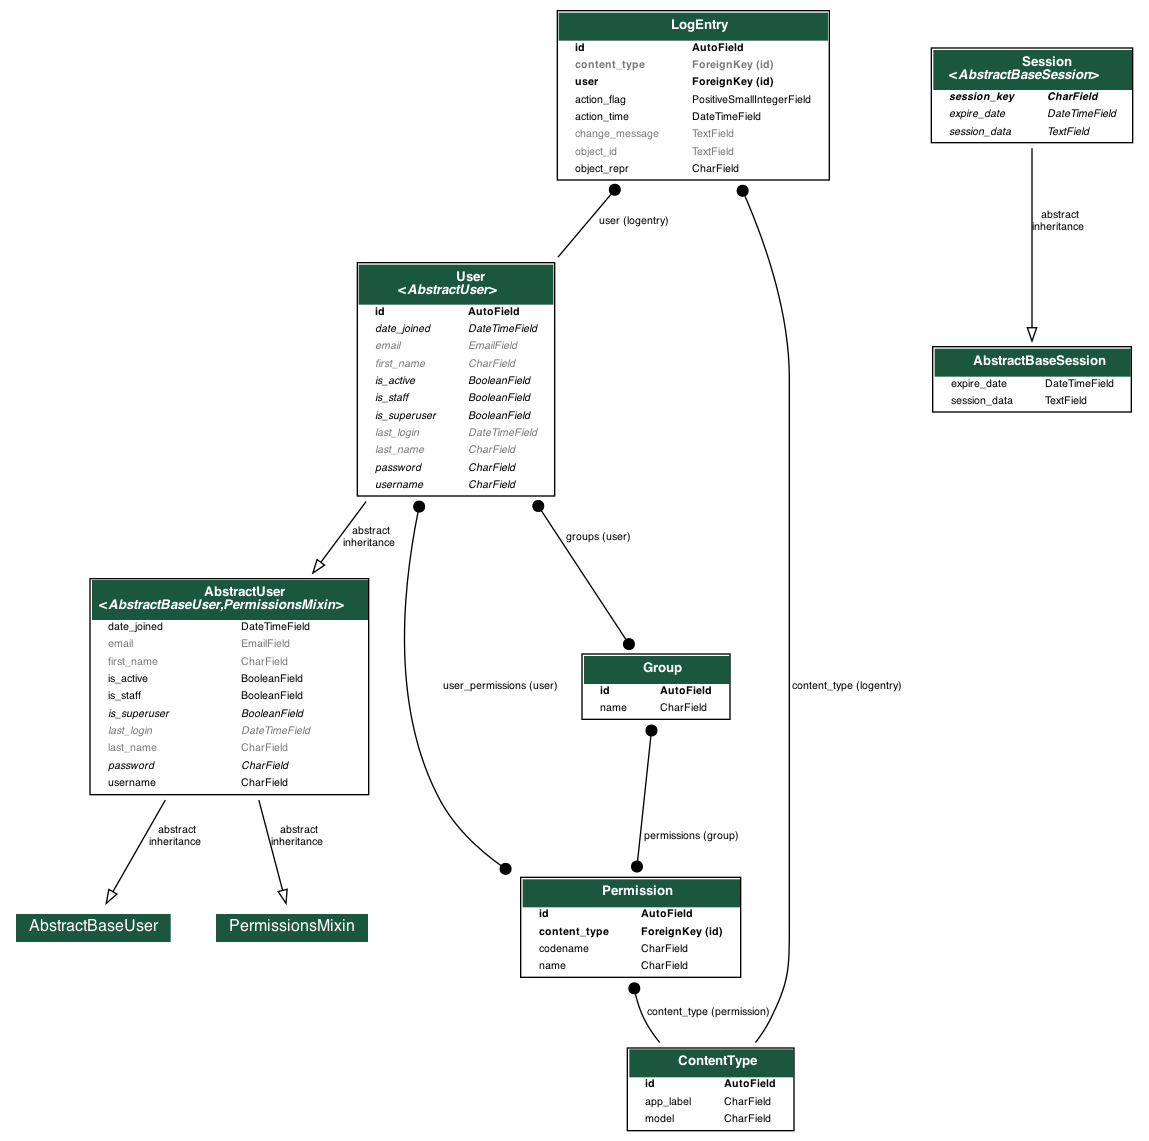
\includegraphics[scale=0.45]{dijagrami/ModelsClassDiagram1.png} %veličina slike u odnosu na originalnu datoteku i pozicija slike
        					\caption{Dijagram razreda modela generične funkcionalnosti}
        					\label{fig:DijagramRazredaModel}
			\end{figure}
			
			\begin{figure}[H]
					\centerfloat
					\advance\leftskip0.7cm
        					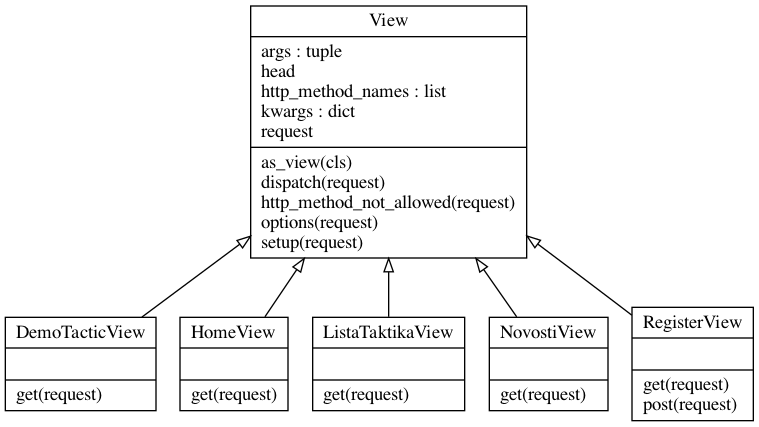
\includegraphics[scale=0.65]{dijagrami/ViewClassDiagram1.png} %veličina slike u odnosu na originalnu datoteku i pozicija slike
        					\caption{Dijagram razreda view-ova generične funkcionalnosti}
        					\label{fig:DijagramRazredaView}
			\end{figure}
			
			\eject
			
			\begin{figure}[H]
					\centerfloat
					\advance\leftskip0.7cm
        					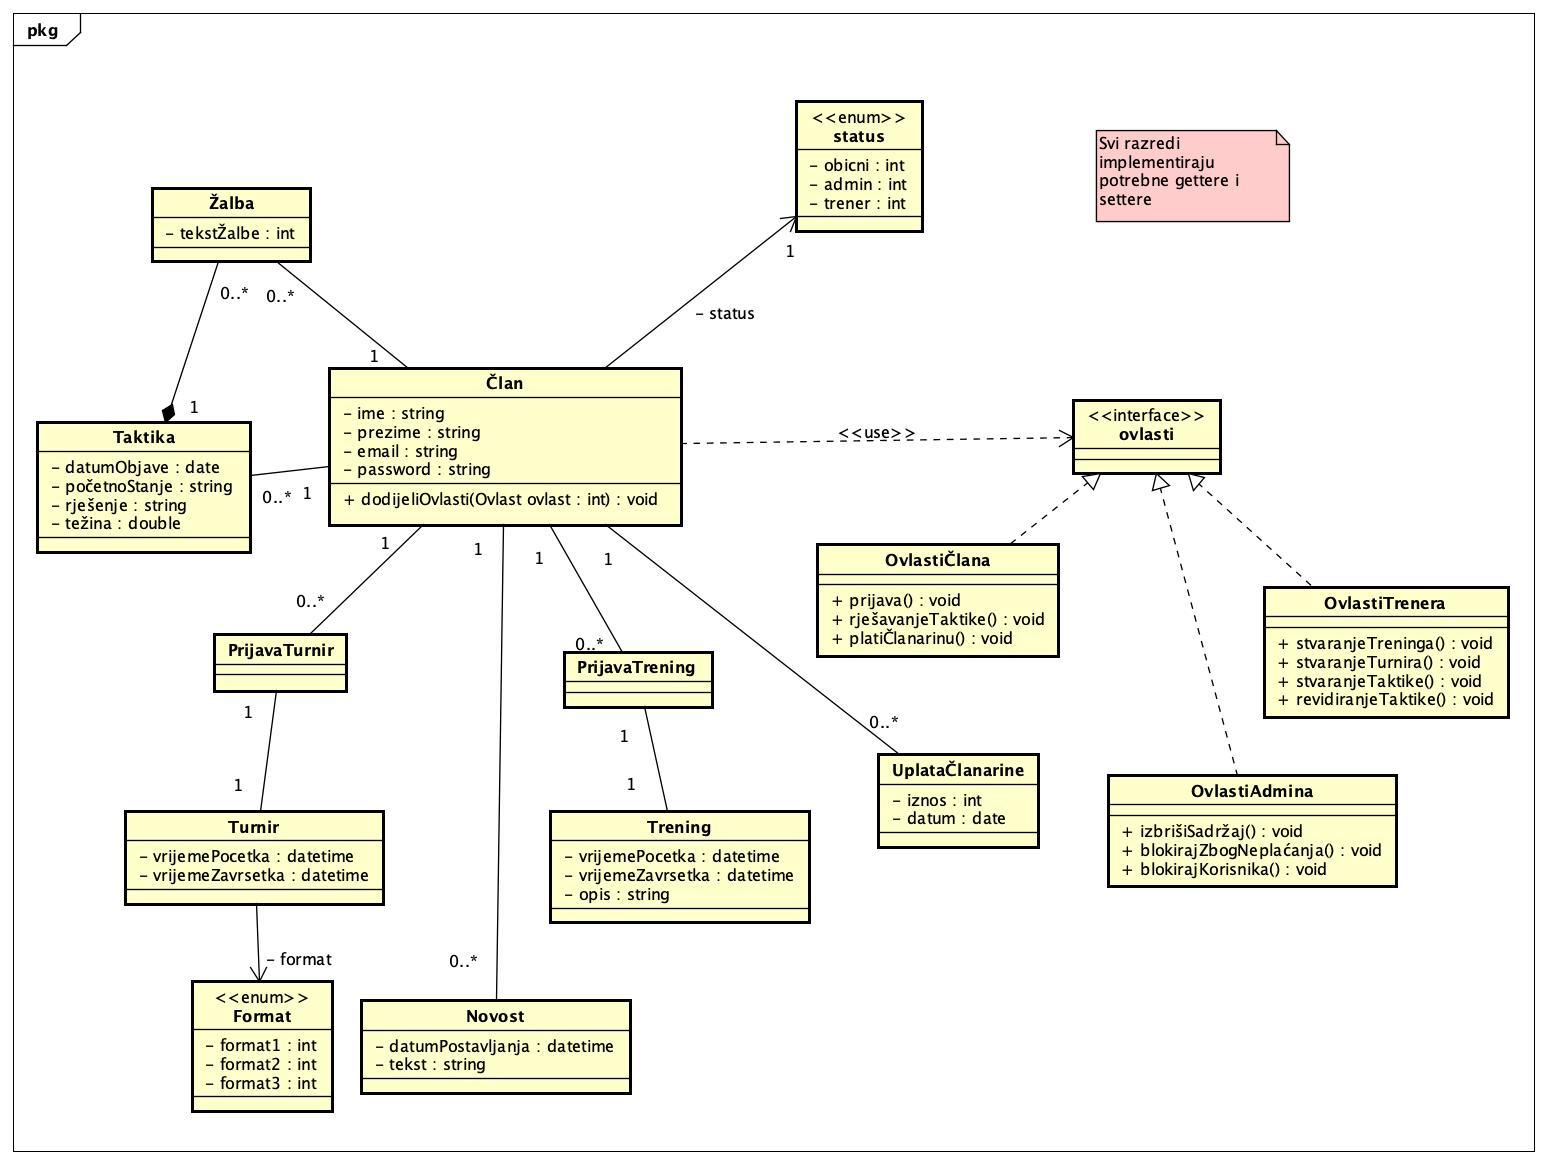
\includegraphics[scale=0.35]{dijagrami/Classdiagram.jpg} %veličina slike u odnosu na originalnu datoteku i pozicija slike
        					\caption{Idejni dijagram razreda}
        					\label{fig:idejniDijagramRazreda}
				\end{figure}

			
			\textbf{\textit{dio 2. revizije}}\\			
			
			\textit{Prilikom druge predaje projekta dijagram razreda i opisi moraju odgovarati stvarnom stanju implementacije}
			
			
			
			\eject
		
		\section{Dijagram stanja}
			
			
			Na slici 4.5 prikazan je dijagram stanja za člana. Pri pokretanju aplikacije, članu se otvara početna stranica. Iz nje može otvoriti stranice "Login“, "Novosti“,  "Profil“, "Registracija“, "Turniri“, "Treninzi“ i "Dnevne taktike“. Na stranici "Login“ član se može prijaviti u svoj račun i u slučaju da ima plaćenu članarinu otvara mu se stranica "Novosti“, a u protivnom "Uplata članarine“ gdje mora uplatiti članarinu.  Odlaskom na "Novosti“ može pregledati sve objavljene novosti u aplikaciji. Iz stranice "Profil“ član može otvoriti stranicu na kojoj može uplatiti članarinu. Preko stranice "Registracija“ može stvoriti novi korisnički raćun. Na stranici "Turniri“ prijavljuje se na novi turnir, a preko stranice "Treninzi“ odabirom trenera i termina prijavljuje se na trening. Iz stranice "Dnevne taktike“ član može otvoriti stranicu "Rang lista“ ili rješavati dnevne taktike. Nakon riješene dnevne taktike ima mogućnost ocjeniti dnevnu taktiku i/ili prijaviti pogrešku u taktici. Član se može odjaviti pritiskom na "Odjavi se“ pri čemu mu se otvara stranica "Novosti“. Pritiskom na "Zatvori stranicu“ izlazi iz aplikacije i završava s radom.
				
			
			
			\begin{figure}[H]
				\centerfloat
				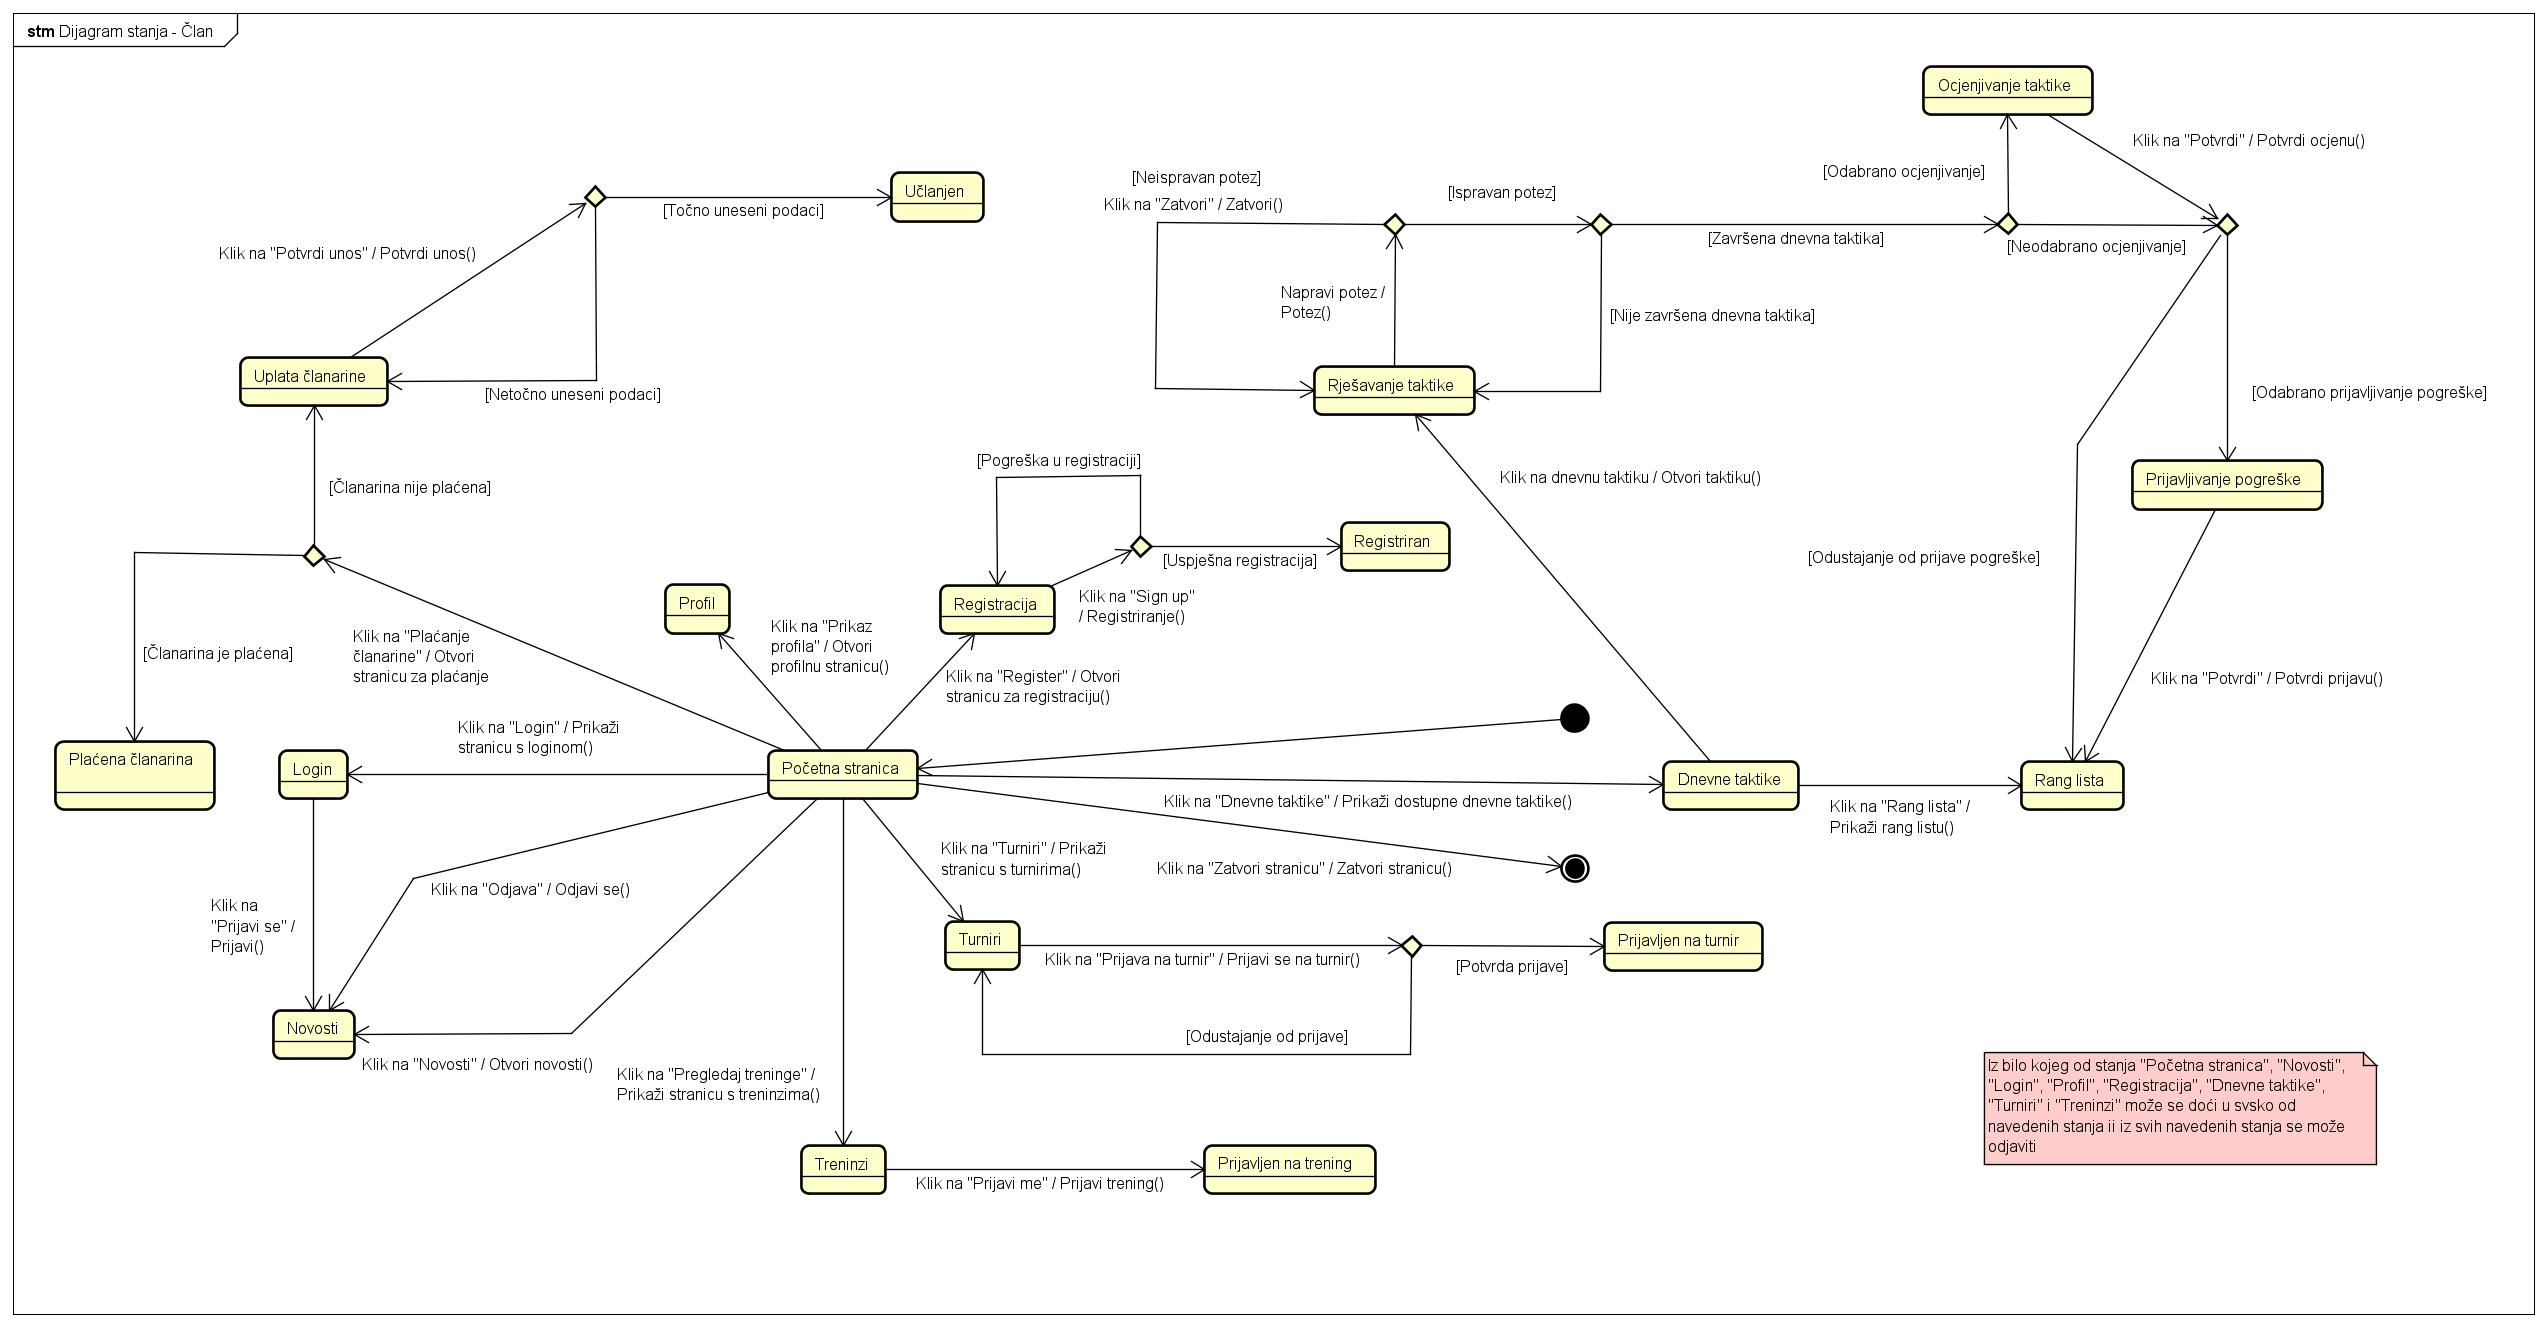
\includegraphics[scale=0.21]{dijagrami/DijagramstanjaClan.jpg} %veličina slike u odnosu na originalnu datoteku i pozicija slike
				\caption{Dijagram stanja za neregistriranog korisnika}
				\label{fig:UC9}
			\end{figure}
			
			\eject
			
			
		\section{Dijagram aktivnosti}
		
		Na slici 4.6 prikazan je proces revidiranja pogreške u taktici. Trener otvara pregled s detaljima o dojavi pogreške u taktici i u ovisnosti o tome je li dojava o pogrešci valjana potvrđuje ili odbija dojavu. U slučaju da prihvati dojavu, taktika se automatski revidira te se rang liste članova također ažuriraju.
			
				\begin{figure}[H]
				\centerfloat
				\includegraphics[scale=0.25]{dijagrami/Dijagram aktivnosti - Revidiranje dojave o pogrešci u taktici.jpg} %veličina slike u odnosu na originalnu datoteku i pozicija slike
				\caption{Dijagram aktivnosti za revidiranje dojave o pogrešci na taktici}
				\label{fig:UC9}
			\end{figure}
			
			\eject
		\section{Dijagram komponenti}
		
			\textbf{\textit{dio 2. revizije}}\\
		
			 \textit{Potrebno je priložiti dijagram komponenti s pripadajućim opisom. Dijagram komponenti treba prikazivati strukturu cijele aplikacije.}